\subsection{Рынок СЭД в Российской Федерации} \label{review_products}

В таблице \ref{table:products} рассмотрены некоторые параметры систем электронного документооборота, представленных на российском рынке \cite{ixbt, evfrat}. Основное внимание уделено универсальности требований к среде исполнения и обеспечению информационной безопасности.

\vspace{\baselineskip}
В целях быстрого захвата рынка большинство СЭД ориентируются на текущие ресурсы предприятий: в качестве целевой ОС используется Microsoft Windows, а базы данных – MS SQL и Oracle. Активное развитие мобильных операционных систем побуждает производителей выпускать клиенты для Android и iOS, а также веб\ndashинтерфейс для управления задачами. Функциональность таких версий обычно урезана: например, они не позволяют добавлять к документу цифровую подпись. При этом для государственных и бюджетных учреждений использование программное обеспечение Microsoft является дополнительной крупной статьёй расхода, избежать которой помогает свободное программное обеспечение.

 \begin{center}
 \renewcommand\multirowsetup{\centering}
 \begin{longtable}[h]{| >{\centering}m{2.5cm} | >{\centering}m{2cm} | >{\centering}m{2cm} | >{\centering}m{2cm} | >{\centering}m{2cm} | >{\centering}m{2cm} | >{\centering}m{2cm} |}
  \captionsetup{justification=raggedright}
  \caption{Существующие системы защиты информации в СЭД} \label{table:products} \tabularnewline
  \hline

 \rowcolor{Gray} СЭД   & Платформа & Поддержка ОС & Встроенное средство контроля целостности & Поддержка различных средств аутентификации & Разграни-чение прав доступа к объектам системы & Выдача прав на время исполнения поручения \tabularnewline \hline \endfirsthead   \hline
 \multicolumn{7}{|c|}{\small\slshape (продолжение таблицы \ref{table:products})}        \tabularnewline \hline
\rowcolor{Gray} СЭД   & Платформа & Поддержка ОС & Встроенное средство контроля целостности & Поддержка различных средств аутентификации & Разграни-чение прав доступа к объектам системы & Выдача прав на время исполнения поручения \tabularnewline \hline
                                              \endhead        \hline
 % \multicolumn{7}{|r|}{\small\slshape продолжение следует}  \tabularnewline \hline
                                              \endfoot        \hline
                                              \endlastfoot

  Босс-референт & \color{Green} Lotus / MS SharePoint / JBOSS & \color{Green} Windows / Linux & \color{Red} \textbf{---} &  \color{Green} \textbf{+} & \color{Green} \textbf{+} & +/-- \tabularnewline \hline

  1С: Документооборот & \color{Red} 1C: Предприятие & \color{Red} Windows & \color{Red} \textbf{---} & +/-- & +/-- & \color{Red} \textbf{---} \tabularnewline \hline

  % CompanyMedia / OfficeMedia & \color{Red} Lotus & \color{Green} Любые & \color{Green} Windows / Linux    \tabularnewline \hline

  % Effect Office & \color{Red} Microsoft & \color{Red} Windows   \tabularnewline \hline

  % LanDocs & \color{Green} Oracle / Microsoft & \color{Red} Windows   \tabularnewline \hline

  Дело (ЭОС) & \color{Green} 1C / MS SharePoint / Oracle & \color{Red} Windows & \color{Red} \textbf{---} & +/--  & +/-- & \color{Green} \textbf{+} \tabularnewline \hline

  DIRECTUM & \color{Red} Microsoft & \color{Red} Windows  & \color{Red} \textbf{---} & +/-- & \color{Green} \textbf{+} & \color{Green} \textbf{+} \tabularnewline \hline

  OPTIMA -- WorkFlow & \color{Green} MS / Oracle & \color{Red} Windows & +/-- & +/-- & +/-- & +/-- \tabularnewline \hline

  DocsVision & \color{Green} MS / Oracle & \color{Red} Windows  & +/-- & \color{Green} \textbf{+} & +/-- & +/-- \tabularnewline \hline

  Е1 ЕВФРАТ & \color{Green} MS / Oracle & \color{Red} Windows & +/-- & +/-- & +/-- & \color{Green} \textbf{+} \tabularnewline \hline

  \rowcolor{Gray} Весовой коэффициент & & 0.15 & 0.28 & 0.145 & 0.24 & 0.185 \tabularnewline \hline
\end{longtable}
\end{center}

\vspace{\baselineskip}
В части обеспечения безопасности обрабатываемой информации все СЭД располагают базовым набором функций:
\begin{itemize}
  \item шифруется канал передачи данных между клиентом и сервером;
  \item используются средства добавления и проверки электронной подписи;
  \item применяются механизмы разграничения доступа.
\end{itemize}

При этом, несмотря на работу с электронной подписью, не все СЭД располагают встроенным средством контроля целостности. В частности, это раскрывается в работе с версиями одного и того же документа: ЭП обычно используется при создании выходного документа, однако в процессе работы контроль целостности и подтверждение авторства отдаётся на откуп внутренним механизмам СЭД, которые не описаны явным образом. В результате можно получить систему, в которой возможен отказ от авторства, а в некоторых случаях и анонимное изменение документа или, наоборот, откат сделанных изменений без должного журналирования.

\vspace{\baselineskip}
Введём комплексный показатель информационной безопасности:
\begin{equation}
  \label{eq:complex}
M = \sum_{i=1}^N k_i \cdot M_i,
\end{equation}
где $k_i$ --- весовой коэффициент, полученный экспертным методом, а $M_i$ -- значение соответствующего фактора.
Оценив таким образом современные СЭД по показателям, описанным в табл. \ref{table:products}, можно получить их наглядное сравнение, представленное на рис. \ref{img:products}.

\begin{figure}[h!]
  \centering
  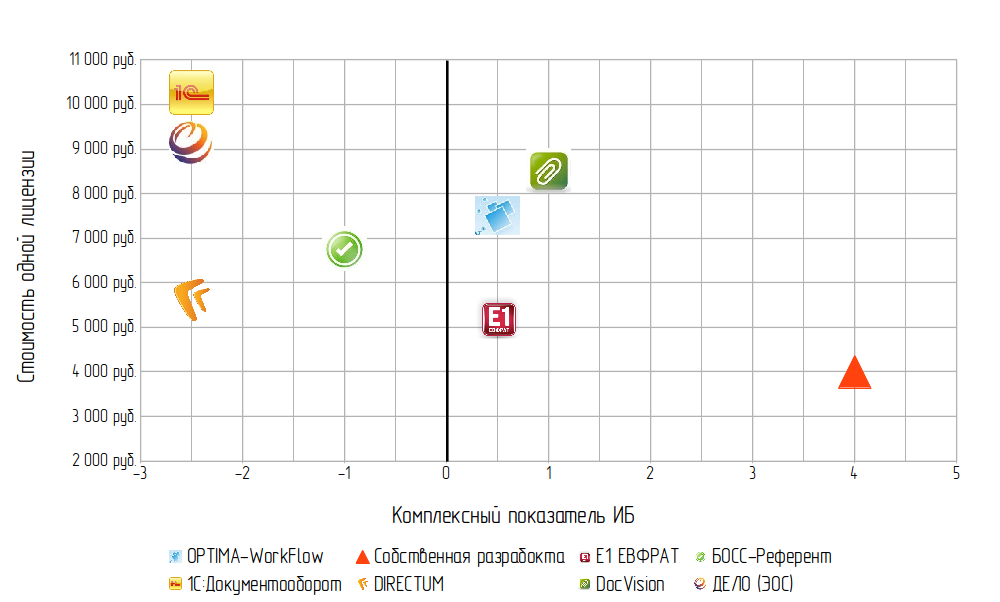
\includegraphics[width=1\textwidth]{products}
  \caption{Сравнение систем электронного документооборота}
  \label{img:products}
\end{figure}
\FloatBarrier

% \vspace{\baselineskip}
% Всё это позволяет сделать вывод о целесообразности создания новой системы электронного документооборота, основанной на открытых технологиях и решающей перечисленные проблемы.